\section{Bedienungsanleitung}
Wir schrieben eine benutzerfreundliche, m"oglichst selbsterkl"arende  Benutzeroberfl"ache f"ur unser Programm. Die wichtigsten Bedienelemente sind im folgendem dokumentiert.

Im Men"upunkt Berechnung gibt es zwei Unterpunkte. Der eine startet eine komplett neue Berechnung, der andere bearbeitet eine bereits bestehende Berechnung. Beide bestehen weitgehend aus denselben Komponenten.

Wir w"ahlen "`Berechnung"'  $\rightarrow$ Untermen"u   "`Neue Berechnung"' $\rightarrow$ Es "offnet sich ein neues Fenster. Mit "`Lade Datei"' kann die entsprechende Eingabedatei ausgew"ahlt werden.
Ist die Karte ausgew"ahlt, hat der Benutzer weitere Einstellungsm"oglichkeiten.
\begin{itemize} 
\item Auf der rechten Seite finden sich die einzelnen Attribute dieser Karte. Der Nutzer kann diese bei jeder neuen Berechnung ver"andern. Somit k"onnen die verschiedenen Einzelattribute, die in den Eingabedatei stehen, unterschiedlich stark gewichtet werden.
\item Mittig unter "`keine Berechnung"' kann die Karte ohne Automaten in unser Hauptfenster eingezeichnet werden. Gewichtskarte bedeutet, dass die Karte die entsprechend gew"ahlten Attribute bereits umsetzt.
\item Auf der linken Seite, kann der Algorithmus ausgew"ahlt werden, mit dem die Automaten auf dieser Karte gesetzt werden. Es gibt zwei Arten von Algorithmen: Die Er"offnungsalgorithmen sowie die Optimierungsalgorithmen. (Unterschiede siehe Algorithmendokumentation)
Bei den Optimierungsalgorithmen, kann die Suchintensit"at eingestellt werden. Ab einer gen"ugend hohen Suchintensit"at, empfiehlt es sich, den Er"offnungsalgorithmus "`Zufall"' zu w"ahlen, da der vorherrgehende Algorithmus keinen signifikanten Einfluss mehr auf die G"ute der L"osung hat. Falls andere als die vorgegebenen oder von uns erzeugten Beispiele verwendet werden (insbesondere bei einer sehr gro"sen Anzahl an Automaten), kann es dennoch sinnvoll sein, den Greedy-Algorithmus zu verwenden.
\item Im unteren Teil kann die Approximationsrate noch ver"andert werden. Die Approximationsrate gibt an, wie stark die Karte verkleinert wird, damit ggf. schnellere Berechnungen erfolgen k"onnen. Zur Auswahl steht die manuelle oder automatische Auswahl der Approximationsrate. Wird sie automatisch gesetzt, so wird diese in Abh"angigkeit des Arbeitsspeichers des entsprechden PCs gew"ahlt. Durch die Auswahl per Hand kann je nach den entsprechenden Bed"urfnissen eine h"ohere oder niedrigere Approximationsrate gew"ahlt werden.
\end{itemize}
Ist die Auswahl getroffen, so wird nach erfolgreicher Eingabe wieder ins Hauptfenster gewechselt. Die angezeigte Karte kann vergr"o"sert oder verkleinert werden. Vielmehr k"onnen die Automaten auch g"anzlich entfernt werden oder zus"atzliche Automaten "uber den Men"upunkt "`Automaten"' gesetzt werden. Will man nicht alle Automaten automatisch setzen lassen, so m"ussen diese entsprechend markiert werden. W"ahlt man nun "`Berechnung"' bearbeiten, so k"onnen die Standpunkte der restlichen Automaten (wie bereits zuvor erw"ahnt) optimiert werden.
Jeder Zustand (wie die Automaten stehen und welches Gewicht sie haben) kann unter dem entsprechenden Men"upunkt gespeichert werden.

\subsection{Eine Beispielberechnung}
Programm Starten  $\rightarrow$ "`Berechnung"' $\rightarrow$ "`Neue Berechnung"' $\rightarrow$ "`Lade Datei"'. Hier w"ahlen wir Hatfield.txt aus. Wir belassen die Attribute alle auf 1, lassen die Approximationsrate automatisch setzen und w"ahlen "`Zeige Pixelkarte und berechne Gewichtskarte"' aus.

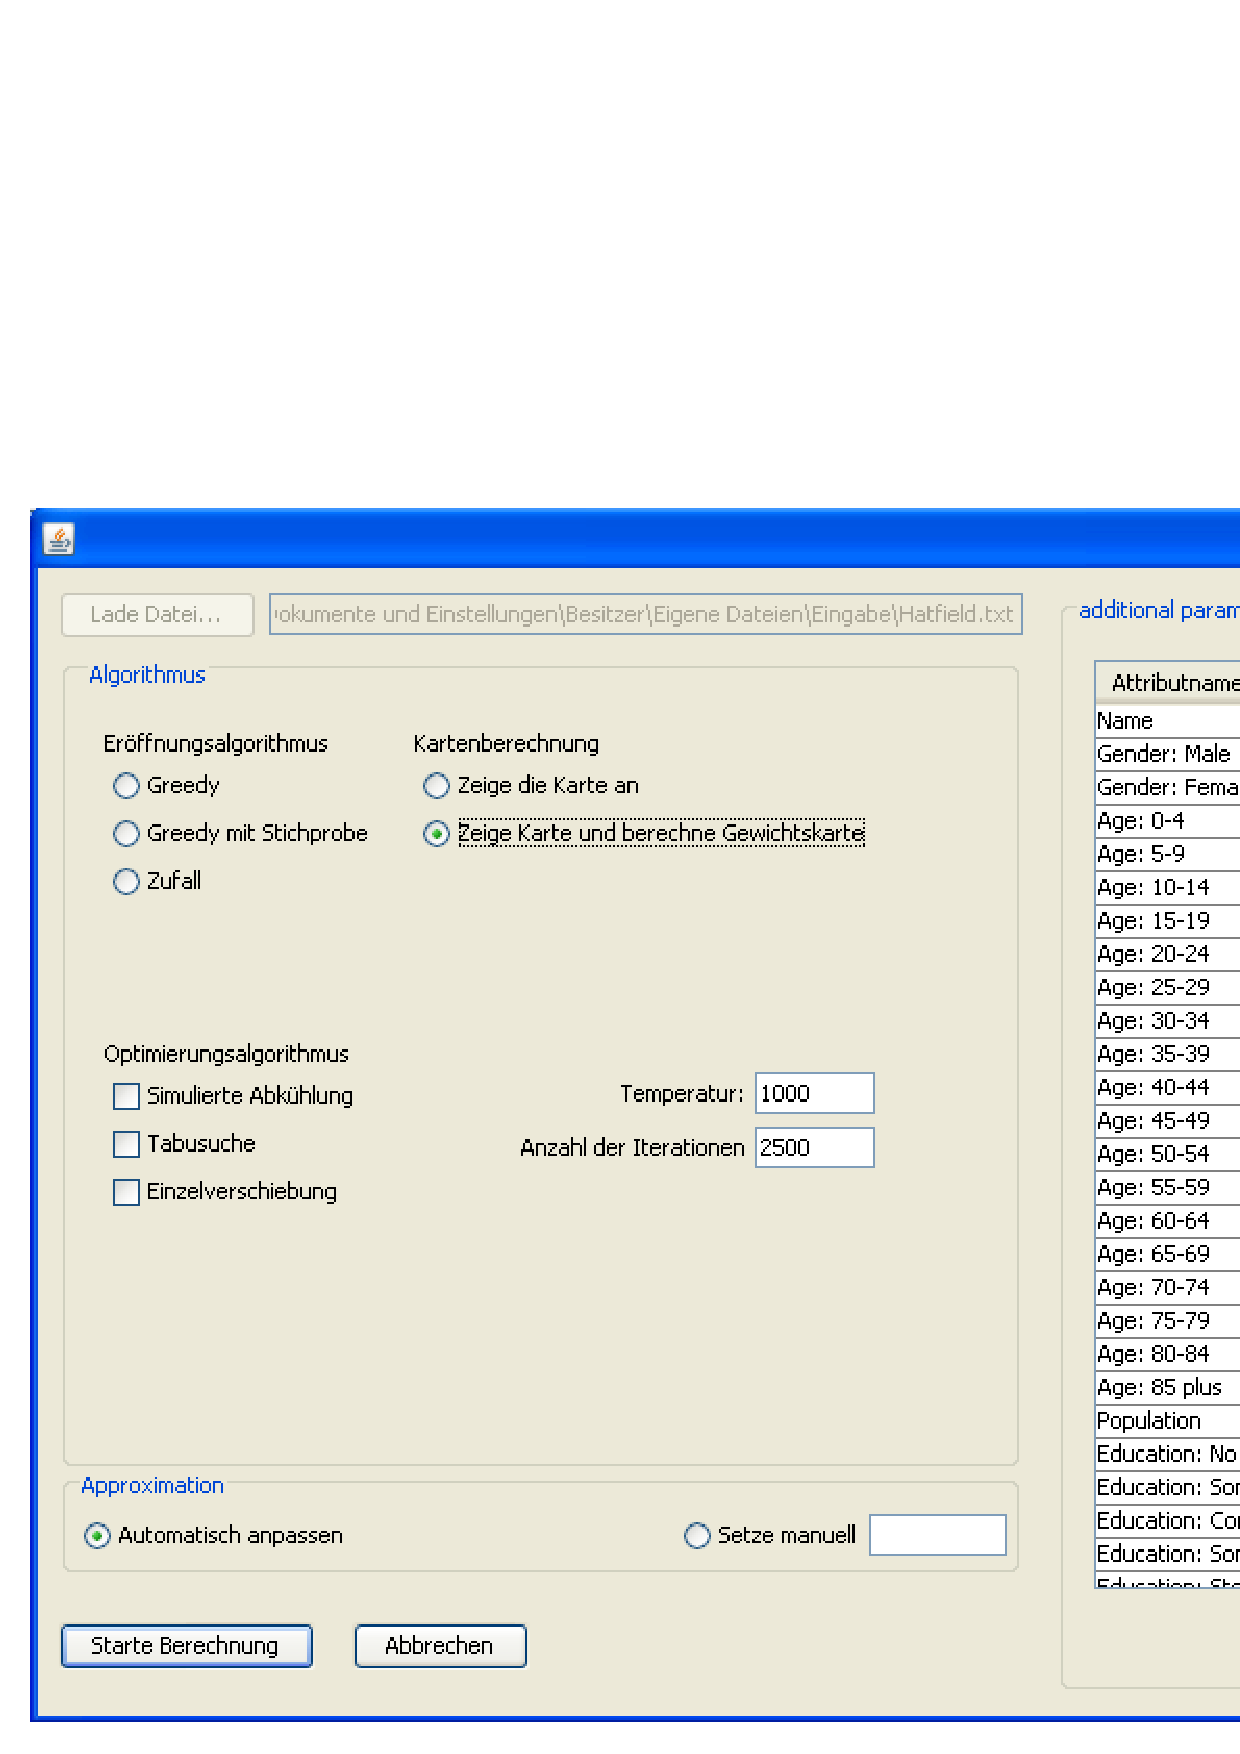
\includegraphics[width=0.5\textwidth]{Gewichtskarte.pdf}

Durch Klicken auf "`Starte Berechnung"' erscheint in etwa folgende Karte.

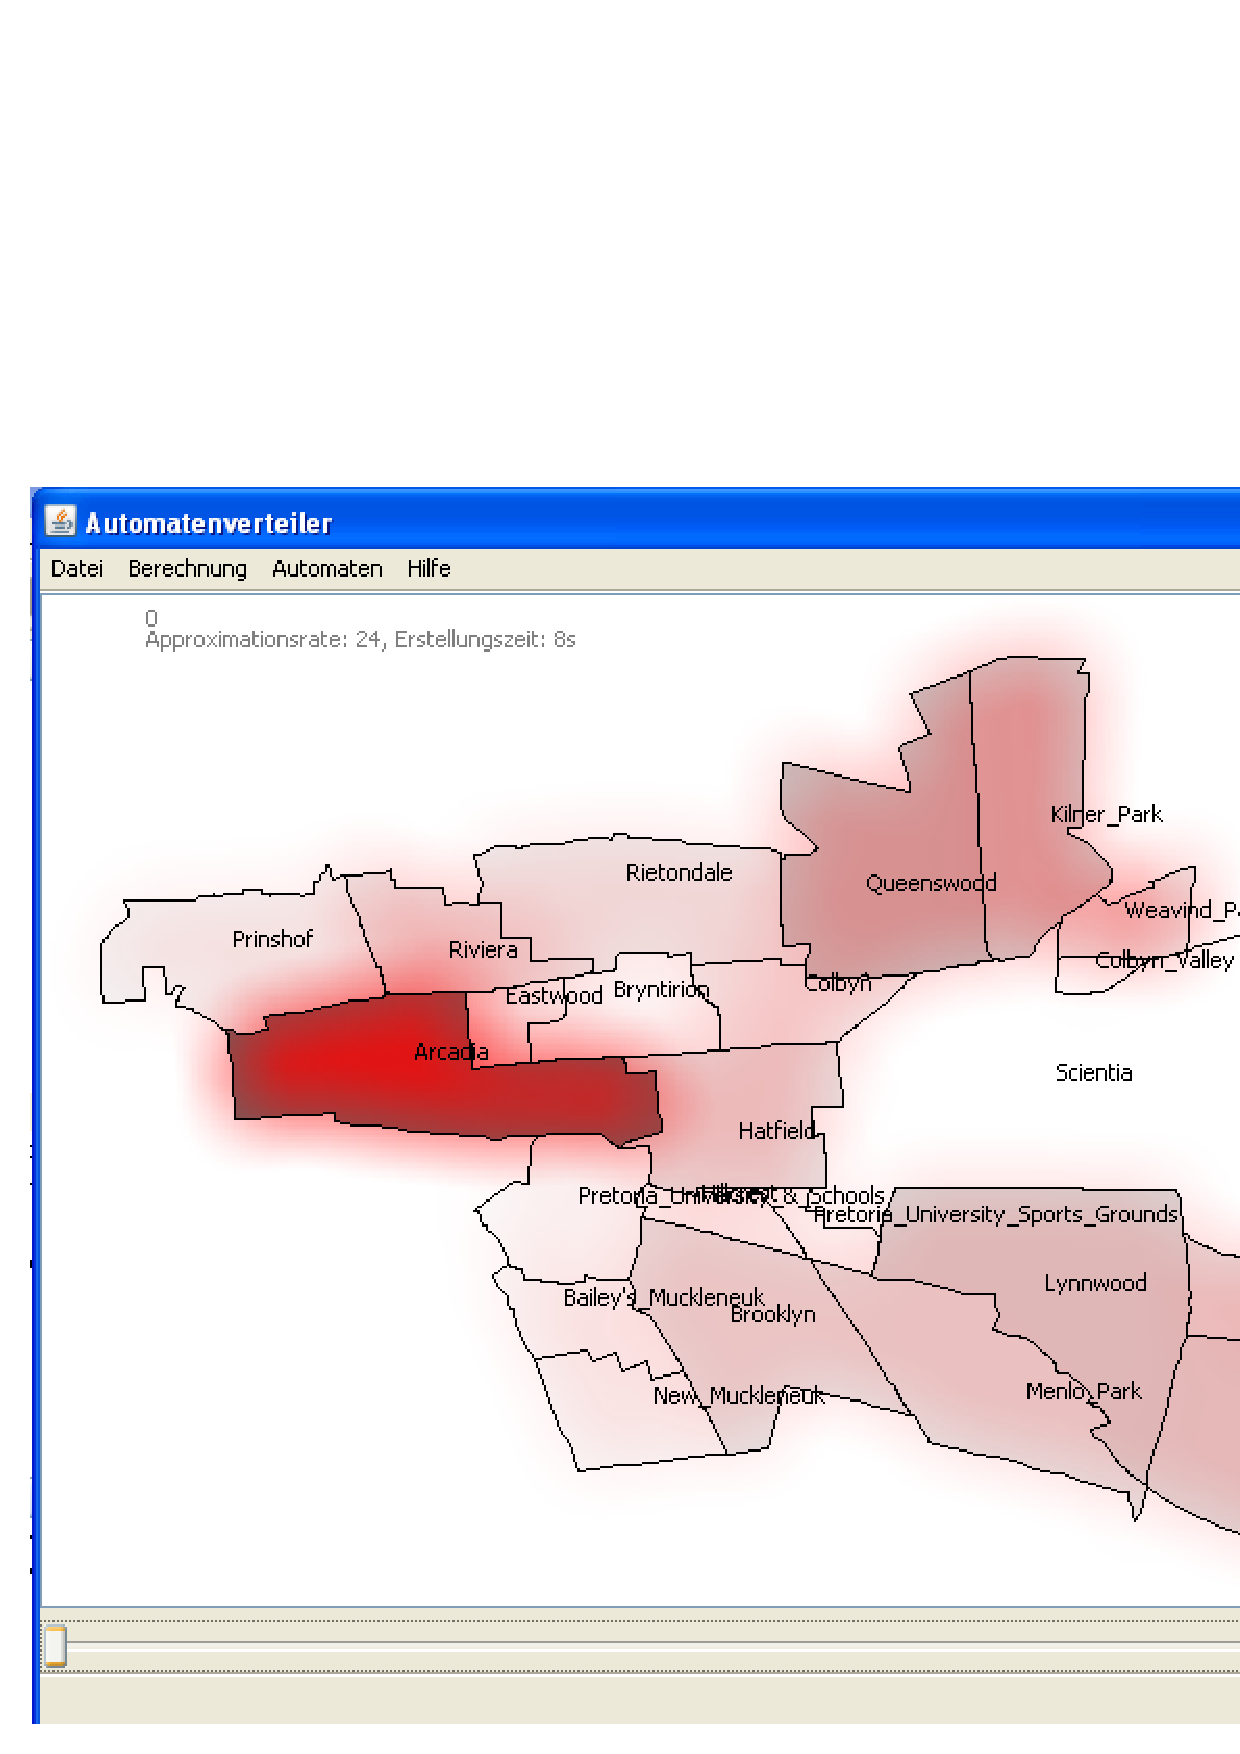
\includegraphics[width=0.5\textwidth]{Gewichtskarte2.pdf}

Nun setzen wir "uber "`Automaten"' $\rightarrow$ "`Neuer Automat"' einen neuen Automaten. Dieser ist fest verankert, kann aber durch entsprechende Men"uauswahl entsperrt werden. Wir f"uhren nun "`Berechnung"'  $\rightarrow$ "`Berechnung bearbeiten "' aus. Hier w"ahlen wir den Greedy-Algorithmus aus und zus"atzlich alle Optimierungsalgorithmen.

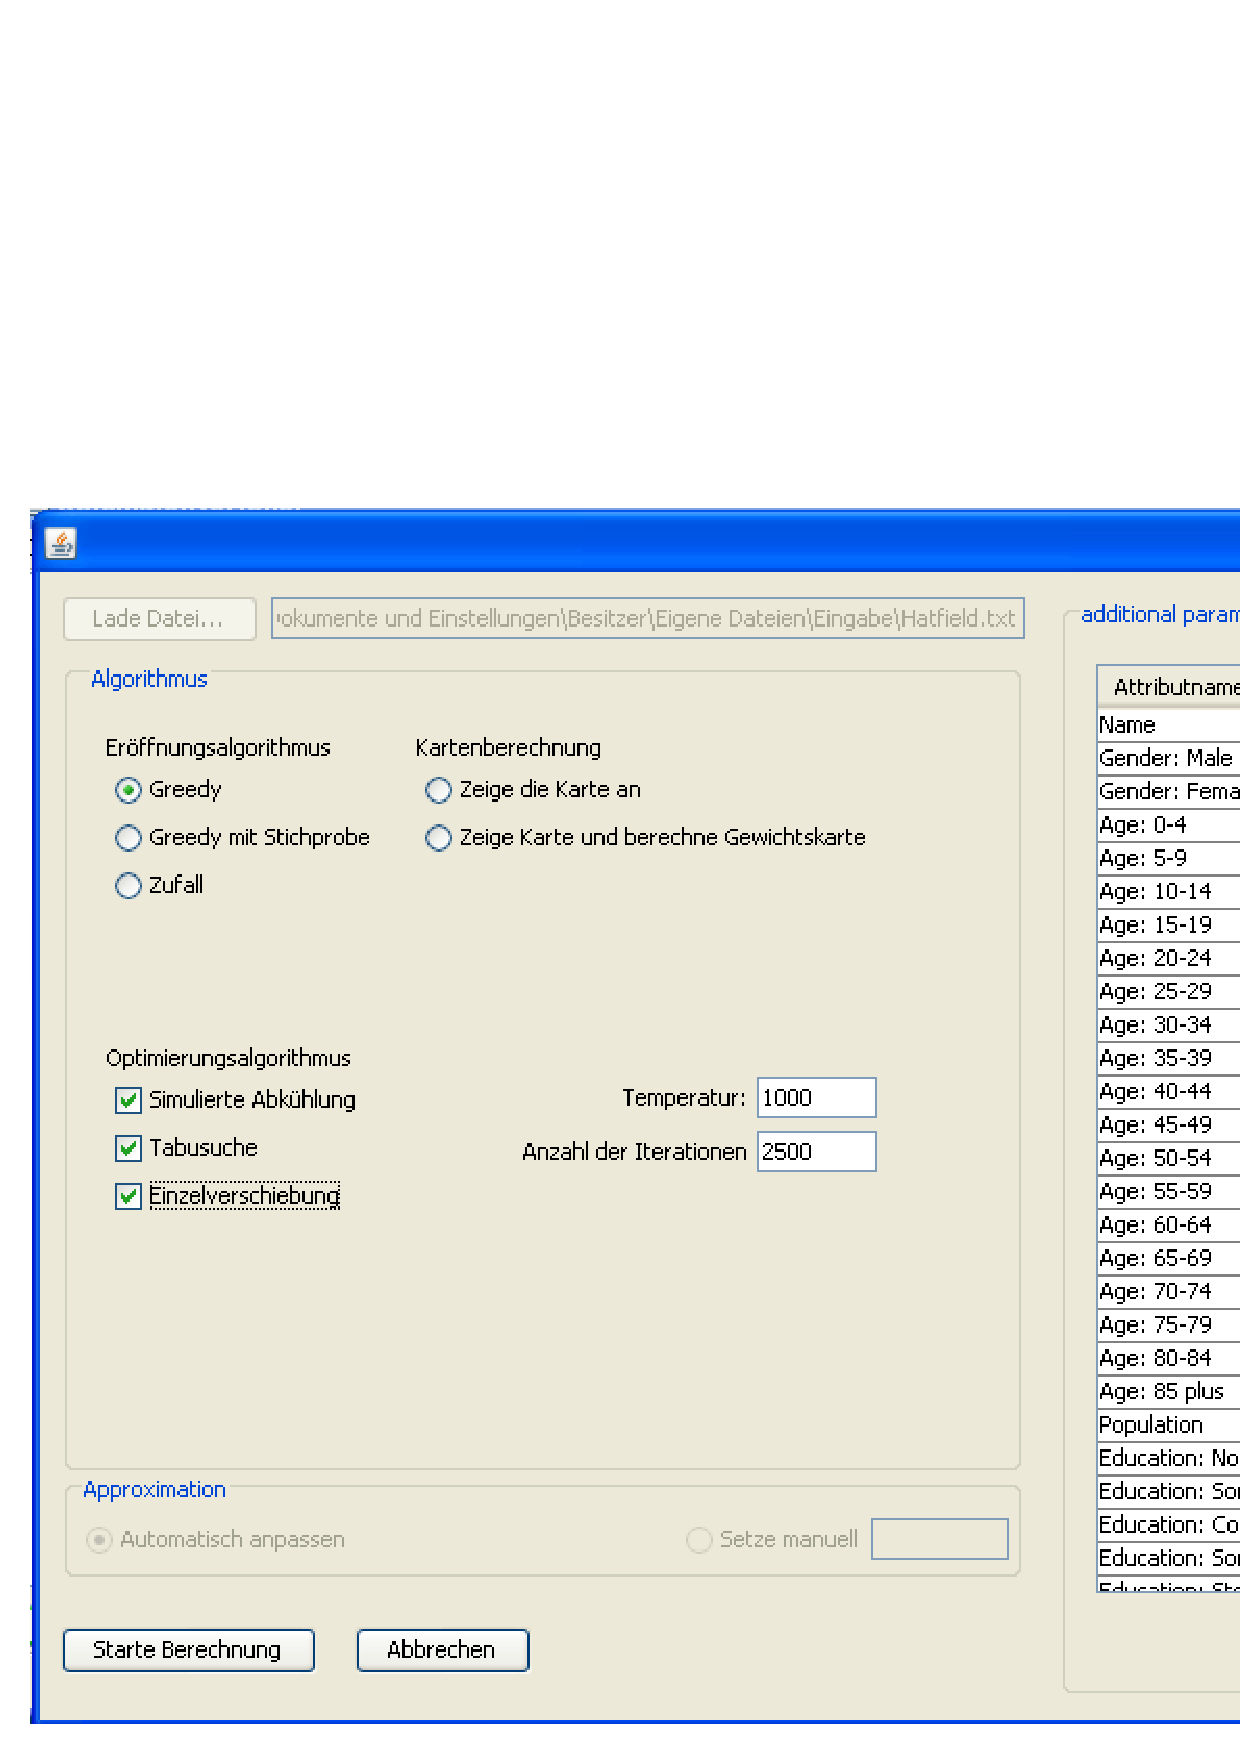
\includegraphics[width=0.5\textwidth] {Allealgos2.pdf}

Sieht dann folgenderma"sen aus.

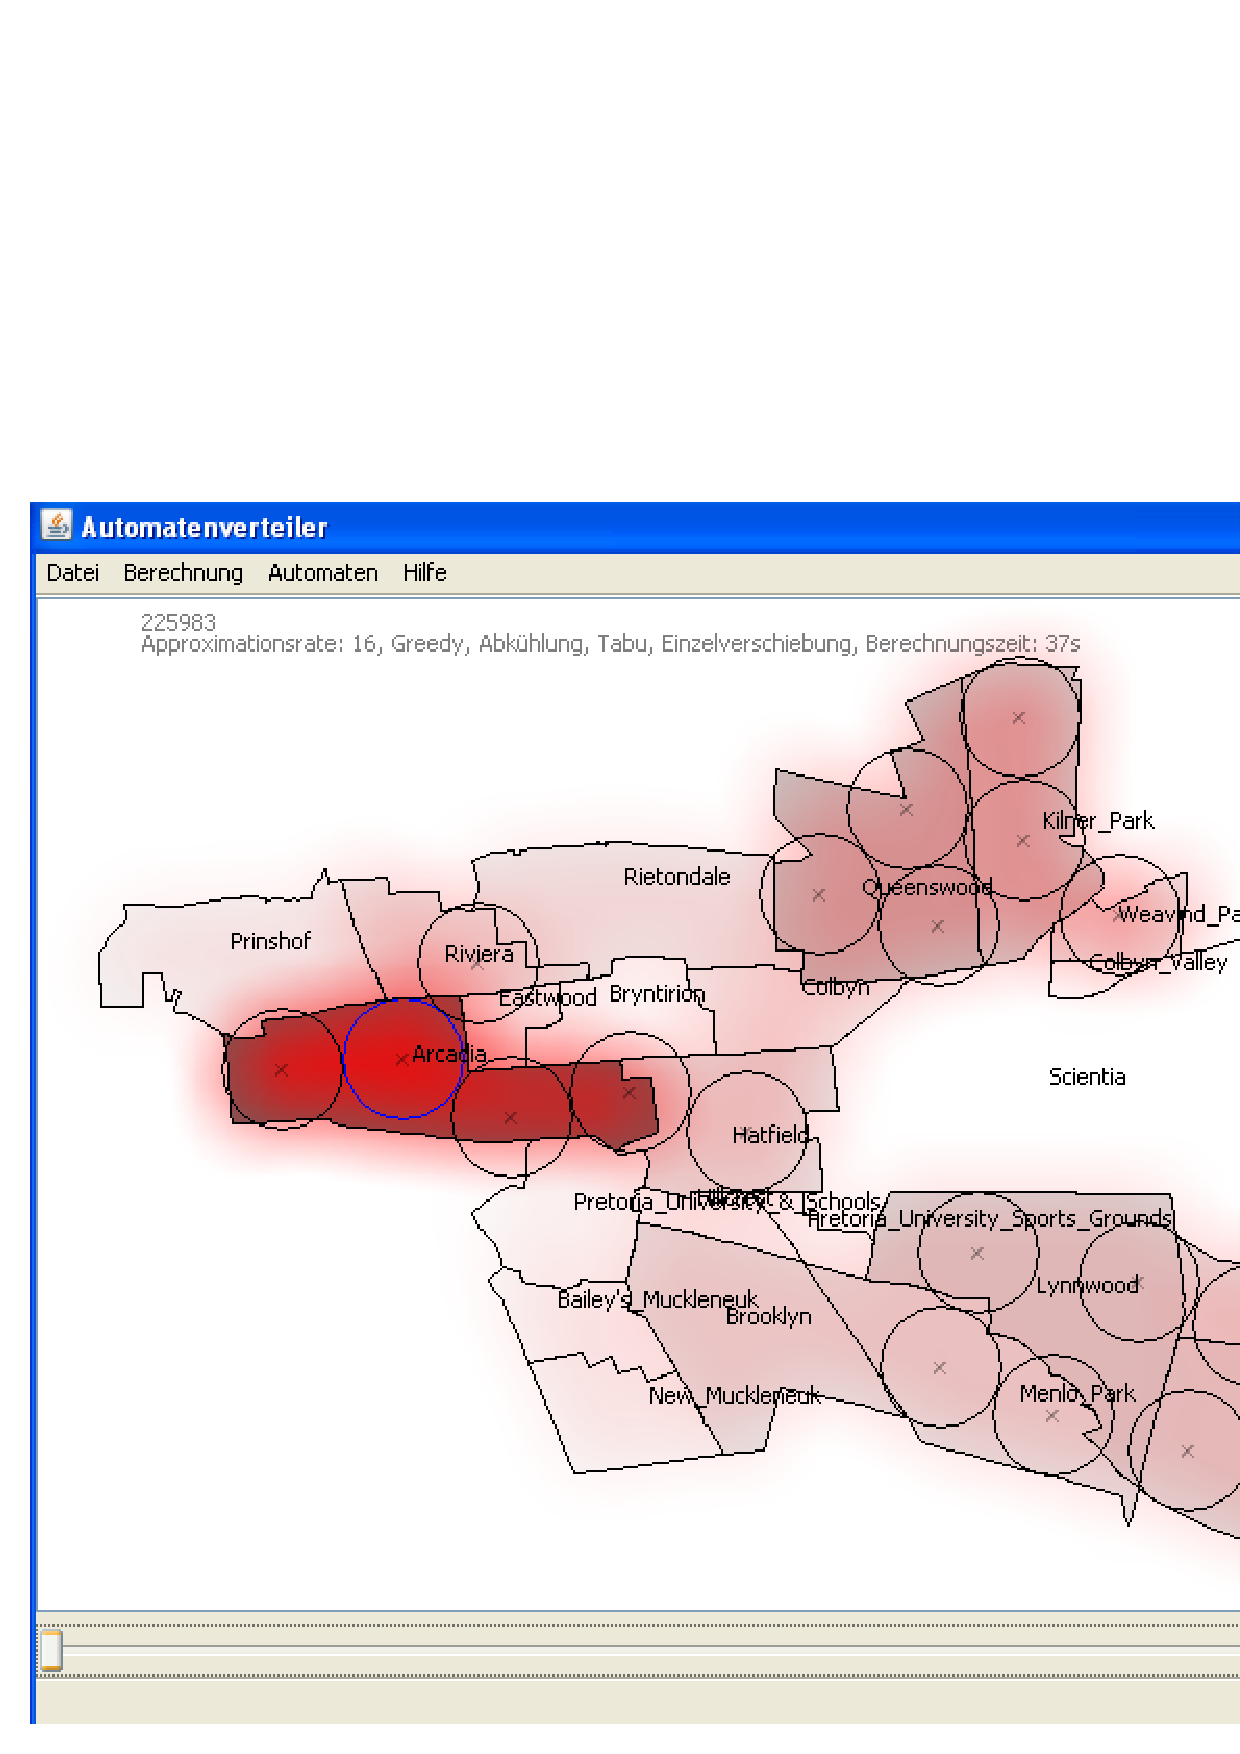
\includegraphics[width=0.5\textwidth] {AlleAlgos.pdf}

Zuletzt speichern wir das Ganze mit "`Datei"' $\rightarrow$ "`Speichern"'.